\section{Sorting}
\scriptsize{Bubble sort}\\ 
{\tiny compare first 2 elements, swap if not in order \\
shift and compare the next 2 elements, again swap if needed \\
when read the end, repeat the process from the beginning unless there were no swaps in the last iteration \\
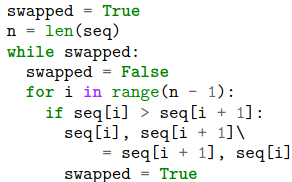
\includegraphics[scale=0.25]{bubble_sort.png}\\
concerns: many swaps, in-place\\
not practical, not used in practice
}\\
\scriptsize{Insertion sort}\\
{\tiny assume the elements arrive one by one, and we have a sorted sequence \\
shift all elements larger than the new one to the right\\
put the new element in its correct place\\
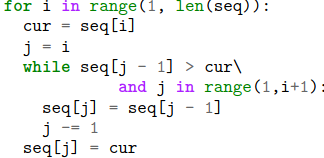
\includegraphics[scale=0.25]{insertion-sort.png}\\
performs reasonably fast for sorting short sequences, on longer sequences, performs worse than more advanced algorithms like merge sort or quick sort\\
in practice faster than bubble sort and selection sort\\
online: sort items as they arrive\\
stable: do not swap elements with equal keys\\
adaptive: faster if order of elements closer to sorted sequence
}\\
\scriptsize{Merge sort}\\
{\tiny split the sequence \\
sort the subsequences\\
merge the sorted lists\\
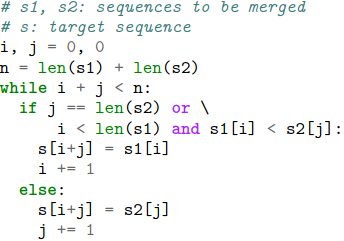
\includegraphics[scale=0.25]{merge-sort_1.png}\\
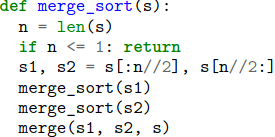
\includegraphics[scale=0.25]{merge-sort_2.png}\\
log n splits\\
particular useful for settings with low random-access memory, or sequential access\\
well-studied, many variants (in-place, non-recursive)
}\\
\scriptsize{Quicksort}\\
{\tiny another popular divide-and-conquer sorting algorithm \\
the big part of the work is done before splitting\\
worst time complexity is O(n**2), but in practice performs better than merge sort on average\\
pick a pivot p, and divide the sequence into 3 parts:\\
L: smaller than p\\
G: larger than p\\
E: equal to p\\
sort L and G recursively\\
combination is simple concatenation\\
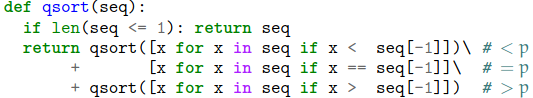
\includegraphics[scale=0.25]{quicksort.png}\\
similar to merge sort, performs O(n) operations at each level in recursion\\
overall complexity is proportional to n*depthOfTree\\
unlike merge sort, no balanced-tree guarantee, in the worst case the depth of the tree can be n, resulting in O(n**2) complexity\\
worst case: when input sequence is sorted\\
randomized quicksort: pick the pivot randomly\\
best case: pick the median of the sequence as pivot, but finding median requires O(nlogn)\\
common apprach: pick 3 values (typically first, middle, last) and select the median\\
can be easily implemented in-place\\
}\\
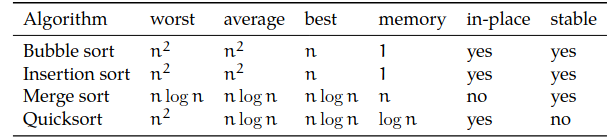
\includegraphics[scale=0.23]{sorting.png}\\
\scriptsize{Bucket sort}\\
{\tiny puts elements of the input into a pre-defined number of ordered 'buckets' \\
elements in each bucket is sorted (typically using insertion sort, worst case O(n**2)\\
can retrieve the sorted elements by visiting each bucket\\
does not compare elements to each other when deciding which bucket to place them\\
in speical cases results in O(n) worst-case complexity (as many buckets as keys)
}\\
\scriptsize{Radix sort}\\
{\tiny sort objects with multiple keys\\
define the order of key pairs as (k1,l1)<(k2,l2) if k1<k2, or k1=k2 and l1<l2, can be generalized to key tuples of any length\\
also known as lexicographic or dictionary order\\
use multiple stable bucket sorts for this purpose
}